% Options for packages loaded elsewhere
\PassOptionsToPackage{unicode}{hyperref}
\PassOptionsToPackage{hyphens}{url}
\PassOptionsToPackage{dvipsnames,svgnames,x11names}{xcolor}
%
\documentclass[
  letterpaper,
  DIV=11,
  numbers=noendperiod]{scrartcl}

\usepackage{amsmath,amssymb}
\usepackage{iftex}
\ifPDFTeX
  \usepackage[T1]{fontenc}
  \usepackage[utf8]{inputenc}
  \usepackage{textcomp} % provide euro and other symbols
\else % if luatex or xetex
  \usepackage{unicode-math}
  \defaultfontfeatures{Scale=MatchLowercase}
  \defaultfontfeatures[\rmfamily]{Ligatures=TeX,Scale=1}
\fi
\usepackage{lmodern}
\ifPDFTeX\else  
    % xetex/luatex font selection
\fi
% Use upquote if available, for straight quotes in verbatim environments
\IfFileExists{upquote.sty}{\usepackage{upquote}}{}
\IfFileExists{microtype.sty}{% use microtype if available
  \usepackage[]{microtype}
  \UseMicrotypeSet[protrusion]{basicmath} % disable protrusion for tt fonts
}{}
\makeatletter
\@ifundefined{KOMAClassName}{% if non-KOMA class
  \IfFileExists{parskip.sty}{%
    \usepackage{parskip}
  }{% else
    \setlength{\parindent}{0pt}
    \setlength{\parskip}{6pt plus 2pt minus 1pt}}
}{% if KOMA class
  \KOMAoptions{parskip=half}}
\makeatother
\usepackage{xcolor}
\setlength{\emergencystretch}{3em} % prevent overfull lines
\setcounter{secnumdepth}{-\maxdimen} % remove section numbering
% Make \paragraph and \subparagraph free-standing
\makeatletter
\ifx\paragraph\undefined\else
  \let\oldparagraph\paragraph
  \renewcommand{\paragraph}{
    \@ifstar
      \xxxParagraphStar
      \xxxParagraphNoStar
  }
  \newcommand{\xxxParagraphStar}[1]{\oldparagraph*{#1}\mbox{}}
  \newcommand{\xxxParagraphNoStar}[1]{\oldparagraph{#1}\mbox{}}
\fi
\ifx\subparagraph\undefined\else
  \let\oldsubparagraph\subparagraph
  \renewcommand{\subparagraph}{
    \@ifstar
      \xxxSubParagraphStar
      \xxxSubParagraphNoStar
  }
  \newcommand{\xxxSubParagraphStar}[1]{\oldsubparagraph*{#1}\mbox{}}
  \newcommand{\xxxSubParagraphNoStar}[1]{\oldsubparagraph{#1}\mbox{}}
\fi
\makeatother

\usepackage{color}
\usepackage{fancyvrb}
\newcommand{\VerbBar}{|}
\newcommand{\VERB}{\Verb[commandchars=\\\{\}]}
\DefineVerbatimEnvironment{Highlighting}{Verbatim}{commandchars=\\\{\}}
% Add ',fontsize=\small' for more characters per line
\usepackage{framed}
\definecolor{shadecolor}{RGB}{241,243,245}
\newenvironment{Shaded}{\begin{snugshade}}{\end{snugshade}}
\newcommand{\AlertTok}[1]{\textcolor[rgb]{0.68,0.00,0.00}{#1}}
\newcommand{\AnnotationTok}[1]{\textcolor[rgb]{0.37,0.37,0.37}{#1}}
\newcommand{\AttributeTok}[1]{\textcolor[rgb]{0.40,0.45,0.13}{#1}}
\newcommand{\BaseNTok}[1]{\textcolor[rgb]{0.68,0.00,0.00}{#1}}
\newcommand{\BuiltInTok}[1]{\textcolor[rgb]{0.00,0.23,0.31}{#1}}
\newcommand{\CharTok}[1]{\textcolor[rgb]{0.13,0.47,0.30}{#1}}
\newcommand{\CommentTok}[1]{\textcolor[rgb]{0.37,0.37,0.37}{#1}}
\newcommand{\CommentVarTok}[1]{\textcolor[rgb]{0.37,0.37,0.37}{\textit{#1}}}
\newcommand{\ConstantTok}[1]{\textcolor[rgb]{0.56,0.35,0.01}{#1}}
\newcommand{\ControlFlowTok}[1]{\textcolor[rgb]{0.00,0.23,0.31}{\textbf{#1}}}
\newcommand{\DataTypeTok}[1]{\textcolor[rgb]{0.68,0.00,0.00}{#1}}
\newcommand{\DecValTok}[1]{\textcolor[rgb]{0.68,0.00,0.00}{#1}}
\newcommand{\DocumentationTok}[1]{\textcolor[rgb]{0.37,0.37,0.37}{\textit{#1}}}
\newcommand{\ErrorTok}[1]{\textcolor[rgb]{0.68,0.00,0.00}{#1}}
\newcommand{\ExtensionTok}[1]{\textcolor[rgb]{0.00,0.23,0.31}{#1}}
\newcommand{\FloatTok}[1]{\textcolor[rgb]{0.68,0.00,0.00}{#1}}
\newcommand{\FunctionTok}[1]{\textcolor[rgb]{0.28,0.35,0.67}{#1}}
\newcommand{\ImportTok}[1]{\textcolor[rgb]{0.00,0.46,0.62}{#1}}
\newcommand{\InformationTok}[1]{\textcolor[rgb]{0.37,0.37,0.37}{#1}}
\newcommand{\KeywordTok}[1]{\textcolor[rgb]{0.00,0.23,0.31}{\textbf{#1}}}
\newcommand{\NormalTok}[1]{\textcolor[rgb]{0.00,0.23,0.31}{#1}}
\newcommand{\OperatorTok}[1]{\textcolor[rgb]{0.37,0.37,0.37}{#1}}
\newcommand{\OtherTok}[1]{\textcolor[rgb]{0.00,0.23,0.31}{#1}}
\newcommand{\PreprocessorTok}[1]{\textcolor[rgb]{0.68,0.00,0.00}{#1}}
\newcommand{\RegionMarkerTok}[1]{\textcolor[rgb]{0.00,0.23,0.31}{#1}}
\newcommand{\SpecialCharTok}[1]{\textcolor[rgb]{0.37,0.37,0.37}{#1}}
\newcommand{\SpecialStringTok}[1]{\textcolor[rgb]{0.13,0.47,0.30}{#1}}
\newcommand{\StringTok}[1]{\textcolor[rgb]{0.13,0.47,0.30}{#1}}
\newcommand{\VariableTok}[1]{\textcolor[rgb]{0.07,0.07,0.07}{#1}}
\newcommand{\VerbatimStringTok}[1]{\textcolor[rgb]{0.13,0.47,0.30}{#1}}
\newcommand{\WarningTok}[1]{\textcolor[rgb]{0.37,0.37,0.37}{\textit{#1}}}

\providecommand{\tightlist}{%
  \setlength{\itemsep}{0pt}\setlength{\parskip}{0pt}}\usepackage{longtable,booktabs,array}
\usepackage{calc} % for calculating minipage widths
% Correct order of tables after \paragraph or \subparagraph
\usepackage{etoolbox}
\makeatletter
\patchcmd\longtable{\par}{\if@noskipsec\mbox{}\fi\par}{}{}
\makeatother
% Allow footnotes in longtable head/foot
\IfFileExists{footnotehyper.sty}{\usepackage{footnotehyper}}{\usepackage{footnote}}
\makesavenoteenv{longtable}
\usepackage{graphicx}
\makeatletter
\newsavebox\pandoc@box
\newcommand*\pandocbounded[1]{% scales image to fit in text height/width
  \sbox\pandoc@box{#1}%
  \Gscale@div\@tempa{\textheight}{\dimexpr\ht\pandoc@box+\dp\pandoc@box\relax}%
  \Gscale@div\@tempb{\linewidth}{\wd\pandoc@box}%
  \ifdim\@tempb\p@<\@tempa\p@\let\@tempa\@tempb\fi% select the smaller of both
  \ifdim\@tempa\p@<\p@\scalebox{\@tempa}{\usebox\pandoc@box}%
  \else\usebox{\pandoc@box}%
  \fi%
}
% Set default figure placement to htbp
\def\fps@figure{htbp}
\makeatother

\KOMAoption{captions}{tableheading}
\makeatletter
\@ifpackageloaded{caption}{}{\usepackage{caption}}
\AtBeginDocument{%
\ifdefined\contentsname
  \renewcommand*\contentsname{Table of contents}
\else
  \newcommand\contentsname{Table of contents}
\fi
\ifdefined\listfigurename
  \renewcommand*\listfigurename{List of Figures}
\else
  \newcommand\listfigurename{List of Figures}
\fi
\ifdefined\listtablename
  \renewcommand*\listtablename{List of Tables}
\else
  \newcommand\listtablename{List of Tables}
\fi
\ifdefined\figurename
  \renewcommand*\figurename{Figure}
\else
  \newcommand\figurename{Figure}
\fi
\ifdefined\tablename
  \renewcommand*\tablename{Table}
\else
  \newcommand\tablename{Table}
\fi
}
\@ifpackageloaded{float}{}{\usepackage{float}}
\floatstyle{ruled}
\@ifundefined{c@chapter}{\newfloat{codelisting}{h}{lop}}{\newfloat{codelisting}{h}{lop}[chapter]}
\floatname{codelisting}{Listing}
\newcommand*\listoflistings{\listof{codelisting}{List of Listings}}
\makeatother
\makeatletter
\makeatother
\makeatletter
\@ifpackageloaded{caption}{}{\usepackage{caption}}
\@ifpackageloaded{subcaption}{}{\usepackage{subcaption}}
\makeatother

\usepackage{bookmark}

\IfFileExists{xurl.sty}{\usepackage{xurl}}{} % add URL line breaks if available
\urlstyle{same} % disable monospaced font for URLs
\hypersetup{
  pdftitle={Kernel Trick and SVM},
  pdfauthor={Cheryl KOUADIO},
  colorlinks=true,
  linkcolor={blue},
  filecolor={Maroon},
  citecolor={Blue},
  urlcolor={Blue},
  pdfcreator={LaTeX via pandoc}}


\title{Kernel Trick and SVM}
\author{Cheryl KOUADIO}
\date{2024-10-04}

\begin{document}
\maketitle


\section{Activity 1 : Kernel Ridge Regression
(KRR)}\label{activity-1-kernel-ridge-regression-krr}

In regression and classification, we often use linear models to predict
the target variable. However, in many cases, the relationship between
the target variable and the explanatory variables is non-linear. In such
cases, we can use the kernel trick whenever there is a scalar product
between the explanatory variables. The kernel trick allows us to
transform the data into a higher-dimensional space where the
relationship is linear.

In this first activity, we will explore the kernel trick to transform
the data and then use a linear model to predict the target variable. In
particular, we will use Kernel ridge regression (KRR) which is a
combination of ridge regression and the kernel trick. The optimization
problem of KRR is given by: \[
\hat \theta = \min_{\theta} \frac{1}{n} \sum_{i=1}^n (y_i - x_i^T\theta)  + \lambda \sum_{j=1}^d \theta_j
\] where \(x_i\) is the \(i\)-th row of the matrix \(X\) and \(y_i\) is
the \(i\)-th element of the vector \(y\). The parameter \(\lambda\) is
the regularization parameter. The solution of the optimization problem
is given by:

\[
\hat \theta = (X^TX + \lambda I_d)^{-1}X^Ty = X^T (X X^T + \lambda I_n)^{-1}y
\]

where \(I_d\) and \(I_n\) are the identity matrix.

In prediction, the target variable is given by: \[
\hat{y}(x^*) = X^T \hat{\theta} = \langle x^*, \hat{\theta} \rangle = \left\langle x^*, \sum_{i=1}^{n} \alpha_i x_i \right\rangle = \sum_{i=1}^{n} \alpha_i \langle x_i, x^* \rangle
\] where \(\alpha_i = \sum_{j=1}^{n} \theta_j x_{ij}\). We easily see
that the prediction is a linear combination of the scalar product
between the test point \(x^*\) and the training points \(x_i\), we can
use the kernel trick to transform the data into a higher-dimensional
space where the relationship is linear. The prediction becomes:

\[
\hat{y}(x^*) = \sum_{i=1}^{n} \alpha_i K(x_i, x^*)
\]

where \(K(x_i, x^*)\) is the kernel function.

\subsection{I. Fit the Kernel Ridge Regression
(KRR)}\label{i.-fit-the-kernel-ridge-regression-krr}

In problem which involves a distance between point, it is a common
practice to normalize the data. In this notebook, we are going to
normalize the data by dividing the time by 60 to convert it from minutes
to hours (and have values between 0 and 1). We are going to use the
\texttt{KernelRidge} class from the \texttt{sklearn} library to fit the
KRR model. We will start by using the Gaussian/RBF kernel which is
defined by: \[
K(x, x') = \exp\left(-\gamma||x - x'||^2\right)
\] where \(\gamma\) is an hyperparameter.

\begin{Shaded}
\begin{Highlighting}[]
\CommentTok{\# Libraries}
\ImportTok{import}\NormalTok{ pandas }\ImportTok{as}\NormalTok{ pd }
\ImportTok{from}\NormalTok{ sklearn.kernel\_ridge }\ImportTok{import}\NormalTok{ KernelRidge}
\ImportTok{from}\NormalTok{ sklearn.model\_selection }\ImportTok{import}\NormalTok{ GridSearchCV}
\ImportTok{from}\NormalTok{ sklearn.metrics }\ImportTok{import}\NormalTok{ mean\_squared\_error}
\ImportTok{from}\NormalTok{ sklearn.model\_selection }\ImportTok{import}\NormalTok{ train\_test\_split}
\ImportTok{import}\NormalTok{ matplotlib.pyplot }\ImportTok{as}\NormalTok{ plt}
\ImportTok{from}\NormalTok{ sklearn.linear\_model }\ImportTok{import}\NormalTok{ RidgeCV}
\ImportTok{from}\NormalTok{ sklearn.neighbors }\ImportTok{import}\NormalTok{ KNeighborsClassifier}
\ImportTok{from}\NormalTok{ sklearn.inspection }\ImportTok{import}\NormalTok{ DecisionBoundaryDisplay}
\ImportTok{from}\NormalTok{ sklearn.svm }\ImportTok{import}\NormalTok{ SVC}
\ImportTok{from}\NormalTok{ sklearn.linear\_model }\ImportTok{import}\NormalTok{ LogisticRegression}
\ImportTok{from}\NormalTok{ sklearn.metrics }\ImportTok{import}\NormalTok{ accuracy\_score, confusion\_matrix, classification\_report}
\CommentTok{\#!pip install umap{-}learn}
\ImportTok{import}\NormalTok{ umap.umap\_ }\ImportTok{as}\NormalTok{ umap}
\ImportTok{import}\NormalTok{ numpy }\ImportTok{as}\NormalTok{ np}
\ImportTok{import}\NormalTok{ math}
\ImportTok{import}\NormalTok{ warnings}
\NormalTok{warnings.filterwarnings(}\StringTok{"ignore"}\NormalTok{)}
\end{Highlighting}
\end{Shaded}

\begin{verbatim}
/Users/cherylkouadio/Library/Python/3.9/lib/python/site-packages/tqdm/auto.py:21: TqdmWarning:

IProgress not found. Please update jupyter and ipywidgets. See https://ipywidgets.readthedocs.io/en/stable/user_install.html
\end{verbatim}

\begin{Shaded}
\begin{Highlighting}[]
\CommentTok{\# Load the data}
\NormalTok{mcycle\_data }\OperatorTok{=}\NormalTok{ pd.read\_csv(}\StringTok{"Data/mcycle.csv"}\NormalTok{)}
\NormalTok{mcycle\_data[}\StringTok{"times"}\NormalTok{] }\OperatorTok{=}\NormalTok{ mcycle\_data[}\StringTok{"times"}\NormalTok{]}\OperatorTok{/}\DecValTok{60} 
\NormalTok{mcycle\_data.describe()}
\end{Highlighting}
\end{Shaded}

\begin{longtable}[]{@{}lll@{}}
\toprule\noalign{}
& times & accel \\
\midrule\noalign{}
\endhead
\bottomrule\noalign{}
\endlastfoot
count & 133.000000 & 133.000000 \\
mean & 0.419649 & -25.545865 \\
std & 0.218868 & 48.322050 \\
min & 0.040000 & -134.000000 \\
25\% & 0.260000 & -54.900000 \\
50\% & 0.390000 & -13.300000 \\
75\% & 0.580000 & 0.000000 \\
max & 0.960000 & 75.000000 \\
\end{longtable}

\begin{Shaded}
\begin{Highlighting}[]
\CommentTok{\# Split the data into train and test sample}
\NormalTok{X }\OperatorTok{=}\NormalTok{ mcycle\_data[[}\StringTok{"times"}\NormalTok{]]}
\NormalTok{y }\OperatorTok{=}\NormalTok{ mcycle\_data[[}\StringTok{"accel"}\NormalTok{]]}
\NormalTok{X\_train, X\_test, y\_train, y\_test }\OperatorTok{=}\NormalTok{ train\_test\_split(X, y, test\_size}\OperatorTok{=}\FloatTok{0.2}\NormalTok{, random\_state}\OperatorTok{=}\DecValTok{42}\NormalTok{)}
\end{Highlighting}
\end{Shaded}

\subsubsection{1. Training and testing RBF kernel ridge
regression}\label{training-and-testing-rbf-kernel-ridge-regression}

Since we have two hyperparameter (\(\gamma\) and \(\lambda\)) to tune,
we can use the GridSearchCV function from scikit-learn to find the best
hyperparameter.

\begin{Shaded}
\begin{Highlighting}[]
\NormalTok{rbf\_krr\_model }\OperatorTok{=}\NormalTok{ KernelRidge(kernel}\OperatorTok{=}\StringTok{"rbf"}\NormalTok{)}
\NormalTok{grid\_eval }\OperatorTok{=}\NormalTok{ np.logspace(}\OperatorTok{{-}}\DecValTok{2}\NormalTok{, }\DecValTok{4}\NormalTok{, }\DecValTok{50}\NormalTok{)}
\NormalTok{param\_grid }\OperatorTok{=}\NormalTok{ \{}\StringTok{"alpha"}\NormalTok{: grid\_eval, }\StringTok{"gamma"}\NormalTok{: grid\_eval\}}
\NormalTok{rbf\_krr\_model\_cv }\OperatorTok{=}\NormalTok{ GridSearchCV(rbf\_krr\_model, param\_grid).fit(X\_train,y\_train)}
\BuiltInTok{print}\NormalTok{(}\SpecialStringTok{f"Best parameters by CV : }\SpecialCharTok{\{}\NormalTok{rbf\_krr\_model\_cv}\SpecialCharTok{.}\NormalTok{best\_params\_}\SpecialCharTok{\}}\SpecialStringTok{"}\NormalTok{)}
\end{Highlighting}
\end{Shaded}

\begin{verbatim}
Best parameters by CV : {'alpha': np.float64(0.07196856730011521), 'gamma': np.float64(35.564803062231285)}
\end{verbatim}

\begin{Shaded}
\begin{Highlighting}[]
\NormalTok{best\_model }\OperatorTok{=}\NormalTok{ KernelRidge(kernel}\OperatorTok{=}\StringTok{"rbf"}\NormalTok{, alpha}\OperatorTok{=}\NormalTok{rbf\_krr\_model\_cv.best\_params\_[}\StringTok{"alpha"}\NormalTok{], gamma}\OperatorTok{=}\NormalTok{rbf\_krr\_model\_cv.best\_params\_[}\StringTok{"gamma"}\NormalTok{])}
\NormalTok{best\_model.fit(X\_train, y\_train)}
\NormalTok{y\_pred }\OperatorTok{=}\NormalTok{ best\_model.predict(X\_test)}

\BuiltInTok{print}\NormalTok{(}\SpecialStringTok{f"Root mean square error: }\SpecialCharTok{\{}\NormalTok{math}\SpecialCharTok{.}\NormalTok{sqrt(mean\_squared\_error(y\_test, y\_pred))}\SpecialCharTok{: .2f\}}\SpecialStringTok{"}\NormalTok{)}
\end{Highlighting}
\end{Shaded}

\begin{verbatim}
Root mean square error:  22.98
\end{verbatim}

\begin{Shaded}
\begin{Highlighting}[]
\CommentTok{\# Sort X\_test and corresponding y\_pred values}
\NormalTok{sorted\_indices }\OperatorTok{=}\NormalTok{ np.argsort(X\_test.values.flatten())}
\NormalTok{X\_test\_sorted }\OperatorTok{=}\NormalTok{ X\_test.values.flatten()[sorted\_indices]}
\NormalTok{y\_pred\_sorted }\OperatorTok{=}\NormalTok{ y\_pred[sorted\_indices]}

\NormalTok{plt.scatter(X\_test, y\_test, color}\OperatorTok{=}\StringTok{"black"}\NormalTok{, label}\OperatorTok{=}\StringTok{"True values"}\NormalTok{)}
\NormalTok{plt.plot(X\_test\_sorted, y\_pred\_sorted, color}\OperatorTok{=}\StringTok{"blue"}\NormalTok{, label}\OperatorTok{=}\StringTok{"Predicted values"}\NormalTok{)}
\NormalTok{plt.title(}\StringTok{"Kernel Ridge Regression"}\NormalTok{)}
\NormalTok{plt.xlabel(}\StringTok{"Input Feature (X)"}\NormalTok{)}
\NormalTok{plt.ylabel(}\StringTok{"Target (y)"}\NormalTok{)}
\NormalTok{plt.legend(loc}\OperatorTok{=}\StringTok{"best"}\NormalTok{)}
\NormalTok{plt.show()}
\end{Highlighting}
\end{Shaded}

\pandocbounded{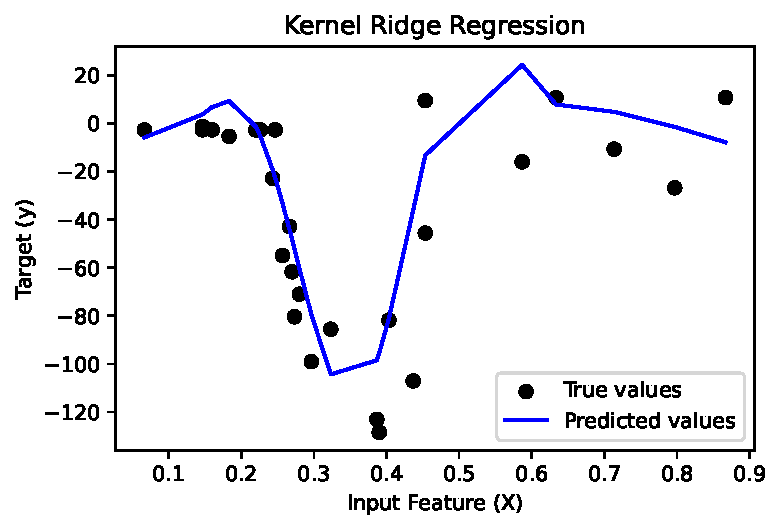
\includegraphics[keepaspectratio]{Tp2_files/figure-pdf/cell-7-output-1.pdf}}

\subsection{II. Ridge regression}\label{ii.-ridge-regression}

Now we are going to use the basic ridge regression to predict the target
variable. There is only one hyperparameter to tune which is the
regularization parameter \(\lambda\).

\begin{Shaded}
\begin{Highlighting}[]
\NormalTok{ridge\_model }\OperatorTok{=}\NormalTok{ RidgeCV(alphas}\OperatorTok{=}\NormalTok{grid\_eval).fit(X\_train, y\_train)}
\NormalTok{y\_pred\_ridge}\OperatorTok{=}\NormalTok{ridge\_model.predict(X\_test)}
\BuiltInTok{print}\NormalTok{( }\SpecialStringTok{f\textquotesingle{}RMSE Ridge regression : }\SpecialCharTok{\{}\NormalTok{math}\SpecialCharTok{.}\NormalTok{sqrt(mean\_squared\_error(y\_test, y\_pred\_ridge)) }\SpecialCharTok{: .2f\}}\SpecialStringTok{\textquotesingle{}}\NormalTok{)}

\CommentTok{\# Plot the results}
\NormalTok{plt.scatter(X\_test, y\_test, color}\OperatorTok{=}\StringTok{"black"}\NormalTok{)}
\NormalTok{plt.plot(X\_test, y\_pred\_ridge, color}\OperatorTok{=}\StringTok{"red"}\NormalTok{)}
\NormalTok{plt.title(}\StringTok{"Ridge Regression"}\NormalTok{)}
\end{Highlighting}
\end{Shaded}

\begin{verbatim}
RMSE Ridge regression :  46.17
\end{verbatim}

\begin{verbatim}
Text(0.5, 1.0, 'Ridge Regression')
\end{verbatim}

\pandocbounded{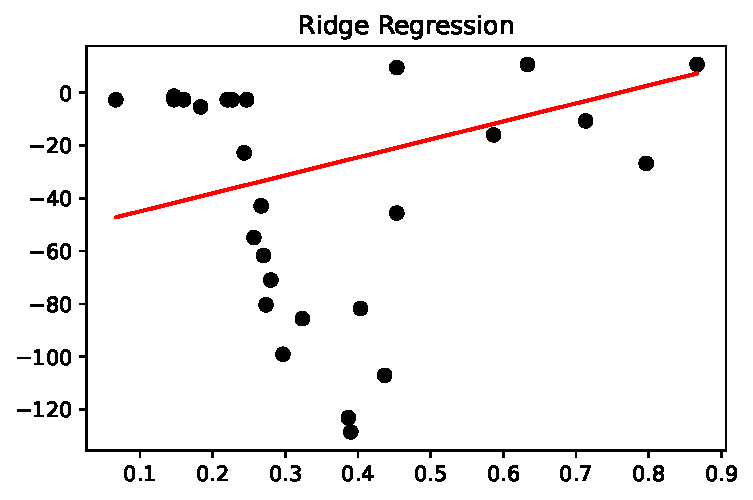
\includegraphics[keepaspectratio]{Tp2_files/figure-pdf/cell-8-output-3.pdf}}

As we can see, the solelly use of the ridge regression is not enough to
predict the target variable. We can try to transform the data by using a
sinusoïdal transformation. If we try a transformation of the covariable
\(x\) by \$\tilde{x} = \frac{\sqrt(2)}{\pi}\cos(\pi x) \$ and apply the
ridge regression, we have a slightly different problem. But still, the
performance of the model is not good.

\begin{Shaded}
\begin{Highlighting}[]
\CommentTok{\# create a function that apply transformation to the features}
\KeywordTok{def}\NormalTok{ apply\_cos(x,j):}
\NormalTok{    pi }\OperatorTok{=}\NormalTok{ np.pi}
    \ControlFlowTok{return}\NormalTok{ np.sqrt(}\DecValTok{2}\NormalTok{)}\OperatorTok{*}\NormalTok{np.cos(j}\OperatorTok{*}\NormalTok{pi}\OperatorTok{*}\NormalTok{x)}\OperatorTok{/}\NormalTok{(j}\OperatorTok{*}\NormalTok{pi)}

\CommentTok{\# perform ridge regression with cosinus modification from j = 1 to 10}
\NormalTok{X\_train\_cos }\OperatorTok{=}\NormalTok{ pd.DataFrame()}
\NormalTok{X\_test\_cos }\OperatorTok{=}\NormalTok{ pd.DataFrame()}
\ControlFlowTok{for}\NormalTok{ j }\KeywordTok{in} \BuiltInTok{range}\NormalTok{(}\DecValTok{1}\NormalTok{,}\DecValTok{11}\NormalTok{):}
\NormalTok{    X\_train\_cos[}\SpecialStringTok{f"X}\SpecialCharTok{\{}\NormalTok{j}\SpecialCharTok{\}}\SpecialStringTok{"}\NormalTok{] }\OperatorTok{=}\NormalTok{ X\_train[}\StringTok{"times"}\NormalTok{].}\BuiltInTok{apply}\NormalTok{(}\KeywordTok{lambda}\NormalTok{ x: apply\_cos(x,j))}
\NormalTok{    X\_test\_cos[}\SpecialStringTok{f"X}\SpecialCharTok{\{}\NormalTok{j}\SpecialCharTok{\}}\SpecialStringTok{"}\NormalTok{] }\OperatorTok{=}\NormalTok{ X\_test[}\StringTok{"times"}\NormalTok{].}\BuiltInTok{apply}\NormalTok{(}\KeywordTok{lambda}\NormalTok{ x: apply\_cos(x,j))}
\end{Highlighting}
\end{Shaded}

\begin{Shaded}
\begin{Highlighting}[]
\CommentTok{\# Train the Ridge regression model}
\NormalTok{ridge\_model1 }\OperatorTok{=}\NormalTok{ RidgeCV(alphas}\OperatorTok{=}\NormalTok{grid\_eval).fit(X\_train\_cos[[}\StringTok{"X1"}\NormalTok{]], y\_train)}
\NormalTok{y\_pred\_ridge1 }\OperatorTok{=}\NormalTok{ ridge\_model1.predict(X\_test\_cos[[}\StringTok{"X1"}\NormalTok{]])}

\NormalTok{rmse\_ridge }\OperatorTok{=}\NormalTok{ math.sqrt(mean\_squared\_error(y\_test, y\_pred\_ridge1))}
\BuiltInTok{print}\NormalTok{(}\SpecialStringTok{f\textquotesingle{}RMSE Ridge regression with x tilde: }\SpecialCharTok{\{}\NormalTok{rmse\_ridge}\SpecialCharTok{:.2f\}}\SpecialStringTok{\textquotesingle{}}\NormalTok{)}
\NormalTok{y\_pred\_ridge1\_sorted }\OperatorTok{=}\NormalTok{ y\_pred\_ridge1[sorted\_indices]}

\NormalTok{plt.scatter(X\_test, y\_test, color}\OperatorTok{=}\StringTok{"black"}\NormalTok{, label}\OperatorTok{=}\StringTok{"True values"}\NormalTok{, s}\OperatorTok{=}\DecValTok{50}\NormalTok{)}
\NormalTok{plt.plot(X\_test\_sorted, y\_pred\_ridge1\_sorted, color}\OperatorTok{=}\StringTok{"red"}\NormalTok{, label}\OperatorTok{=}\StringTok{"Predicted values (Ridge)"}\NormalTok{, linewidth}\OperatorTok{=}\DecValTok{2}\NormalTok{)}
\NormalTok{plt.title(}\StringTok{"Ridge Regression"}\NormalTok{)}
\NormalTok{plt.xlabel(}\StringTok{"Input Feature (X)"}\NormalTok{)}
\NormalTok{plt.ylabel(}\StringTok{"Target (y)"}\NormalTok{)}
\NormalTok{plt.legend(loc}\OperatorTok{=}\StringTok{"best"}\NormalTok{)}
\NormalTok{plt.show()}
\end{Highlighting}
\end{Shaded}

\begin{verbatim}
RMSE Ridge regression with x tilde: 45.87
\end{verbatim}

\pandocbounded{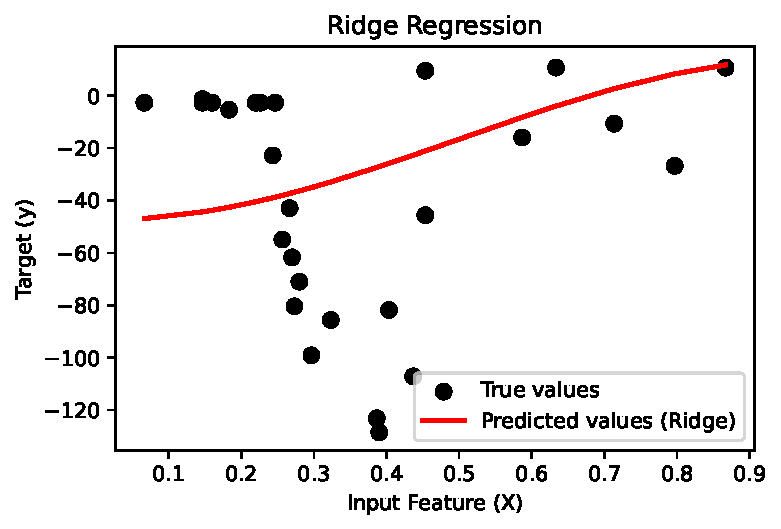
\includegraphics[keepaspectratio]{Tp2_files/figure-pdf/cell-10-output-2.pdf}}

Even though, the only transformation applied is the cosinus
transformation, the RMSE is lower than the RMSE of the simple Ridge
Regression. This is due to the fact that the cosinus transformation is
able to capture a little bit of the periodicity of the data. Let's try
to use many sinusoidal transformation to see if we can improve the
performance of the model. We will fit y using
\(\tilde{x} = \left[ \frac{\sqrt(2)}{J\pi}\cos(J\pi x)  \right]_{J=1,\dots,10}\)

\begin{Shaded}
\begin{Highlighting}[]
\CommentTok{\# New ridge with many transformated features}
\NormalTok{ridge\_model2 }\OperatorTok{=}\NormalTok{ RidgeCV(alphas}\OperatorTok{=}\NormalTok{grid\_eval).fit(X\_train\_cos, y\_train)}
\NormalTok{y\_pred\_ridge2 }\OperatorTok{=}\NormalTok{ ridge\_model2.predict(X\_test\_cos)}
\NormalTok{y\_pred\_ridge2\_sorted }\OperatorTok{=}\NormalTok{ y\_pred\_ridge2[sorted\_indices]}
\BuiltInTok{print}\NormalTok{( }\SpecialStringTok{f\textquotesingle{}RMSE Ridge regression : }\SpecialCharTok{\{}\NormalTok{math}\SpecialCharTok{.}\NormalTok{sqrt(mean\_squared\_error(y\_test, y\_pred\_ridge2))}\SpecialCharTok{: .2f\}}\SpecialStringTok{\textquotesingle{}}\NormalTok{)}

\CommentTok{\# Plot the results}
\NormalTok{plt.scatter(X\_test, y\_test, color}\OperatorTok{=}\StringTok{"black"}\NormalTok{,label}\OperatorTok{=}\StringTok{"True values"}\NormalTok{)}
\NormalTok{plt.plot(X\_test\_sorted, y\_pred\_ridge2\_sorted,color}\OperatorTok{=}\StringTok{"red"}\NormalTok{,label}\OperatorTok{=}\StringTok{"Predicted values (Ridge)"}\NormalTok{)}
\NormalTok{plt.title(}\StringTok{"Ridge Regression"}\NormalTok{)}
\NormalTok{plt.xlabel(}\StringTok{"Input Feature (X)"}\NormalTok{)}
\NormalTok{plt.ylabel(}\StringTok{"Target (y)"}\NormalTok{)}
\NormalTok{plt.legend(loc}\OperatorTok{=}\StringTok{"best"}\NormalTok{)}
\NormalTok{plt}
\end{Highlighting}
\end{Shaded}

\begin{verbatim}
RMSE Ridge regression :  22.96
\end{verbatim}

\pandocbounded{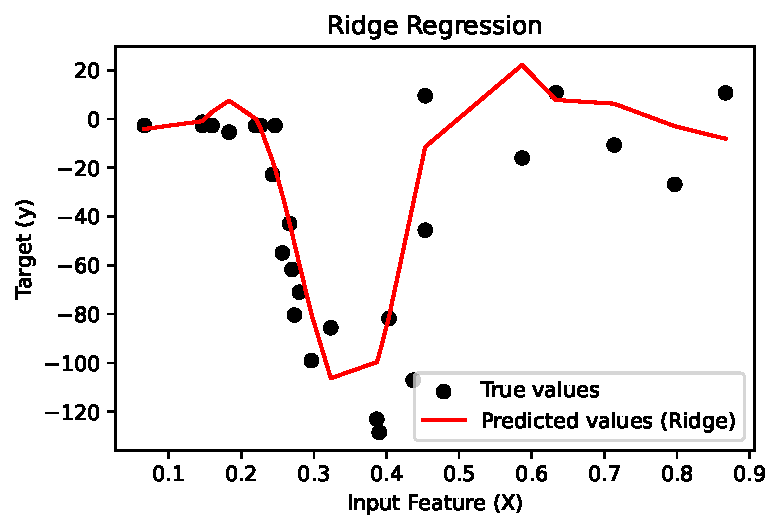
\includegraphics[keepaspectratio]{Tp2_files/figure-pdf/cell-11-output-2.pdf}}

We observe that the more we increase the number of transformations, the
more the performance of the model is improved and close to the
performance of the kernel ridge regression using the gaussian kernel.
The performance of the model is similar to the performance of the kernel
ridge regression. This is due to the fact that the kernel ridge
regression is equivalent to use an infinite number of transformations on
the features. It is hence useful to use the kernel trick when we have a
non-linear relationship between the target variable and the features.

\subsection{III. Insigths :}\label{iii.-insigths}

Linear regression with such sinusoidal transformation is equivalent to
the kernel ridge regression with a specific kernel : the sobolev kernel.
The sobolev kernel is defined by: \[
K(x, x') = 1 + B_1(x)B_2(x') + \frac{1}{2}B_2(|x-x'|) = 1 + B_2(\frac{|x-x'|}{2}) + B_2(\frac{x+x'}{2})
\]

where \(B_1 = x - 1/2\) and \(B_2 = x^2 - x - 1/6\).

Using the fourier series expansion for \(x \in [0,1]\), we have : \[
B_2(x) = \sum_{k=1}^{\infty} \frac{\cos(2k\pi x)}{(k\pi)^2}
\]

\subsubsection{Kernel de sobolev}\label{kernel-de-sobolev}

\begin{Shaded}
\begin{Highlighting}[]
\KeywordTok{def}\NormalTok{ sobolev\_kernel(x,y):}
    \KeywordTok{def}\NormalTok{ B2(x):}
        \ControlFlowTok{return}\NormalTok{ x}\OperatorTok{**}\DecValTok{2} \OperatorTok{{-}}\NormalTok{ x }\OperatorTok{+} \DecValTok{1}\OperatorTok{/}\DecValTok{6}
    
    \KeywordTok{def}\NormalTok{ B1(x):}
        \ControlFlowTok{return}\NormalTok{ x }\OperatorTok{{-}} \DecValTok{1}\OperatorTok{/}\DecValTok{2}
    
    \ControlFlowTok{return} \DecValTok{1}\OperatorTok{+}\NormalTok{ B2(}\BuiltInTok{abs}\NormalTok{(x}\OperatorTok{{-}}\NormalTok{y)}\OperatorTok{/}\DecValTok{2}\NormalTok{) }\OperatorTok{+}\NormalTok{ B2((x}\OperatorTok{+}\NormalTok{y)}\OperatorTok{/}\DecValTok{2}\NormalTok{)}
\end{Highlighting}
\end{Shaded}

\begin{Shaded}
\begin{Highlighting}[]
\NormalTok{krr\_model\_sobolev }\OperatorTok{=}\NormalTok{ KernelRidge(kernel}\OperatorTok{=}\NormalTok{sobolev\_kernel)}
\NormalTok{param\_grid }\OperatorTok{=}\NormalTok{ \{}\StringTok{"alpha"}\NormalTok{: grid\_eval\}}
\NormalTok{grid\_sobolev }\OperatorTok{=}\NormalTok{ GridSearchCV(krr\_model\_sobolev, param\_grid).fit(X\_train,y\_train)}
\NormalTok{grid\_sobolev.best\_params\_}
\end{Highlighting}
\end{Shaded}

\begin{verbatim}
{'alpha': np.float64(0.07196856730011521)}
\end{verbatim}

\begin{Shaded}
\begin{Highlighting}[]
\CommentTok{\# compute rmse}
\CommentTok{\# best\_sobolev\_krr = KernelRidge(kernel=sobolev\_kernel, alpha=grid\_sobolev.best\_params\_["alpha"])}
\CommentTok{\# best\_sobolev\_krr.fit(X\_train, y\_train)}
\NormalTok{y\_pred\_sobolev }\OperatorTok{=}\NormalTok{ grid\_sobolev.predict(X\_test)}
\NormalTok{y\_pred\_sobolev\_sorted }\OperatorTok{=}\NormalTok{ y\_pred\_sobolev[sorted\_indices]}
\BuiltInTok{print}\NormalTok{( }\SpecialStringTok{f\textquotesingle{}Root mean square error : }\SpecialCharTok{\{}\NormalTok{math}\SpecialCharTok{.}\NormalTok{sqrt(mean\_squared\_error(y\_test, y\_pred\_sobolev\_sorted))}\SpecialCharTok{: .2f\}}\SpecialStringTok{\textquotesingle{}}\NormalTok{)}


\CommentTok{\# Plot the results}
\NormalTok{plt.scatter(X\_test, y\_test, color}\OperatorTok{=}\StringTok{"black"}\NormalTok{)}
\NormalTok{plt.plot(X\_test\_sorted, y\_pred\_sobolev\_sorted,color}\OperatorTok{=}\StringTok{"red"}\NormalTok{)}
\NormalTok{plt.title(}\StringTok{"Sobolev Kernel Ridge Regression"}\NormalTok{)}
\end{Highlighting}
\end{Shaded}

\begin{verbatim}
Root mean square error :  61.98
\end{verbatim}

\begin{verbatim}
Text(0.5, 1.0, 'Sobolev Kernel Ridge Regression')
\end{verbatim}

\pandocbounded{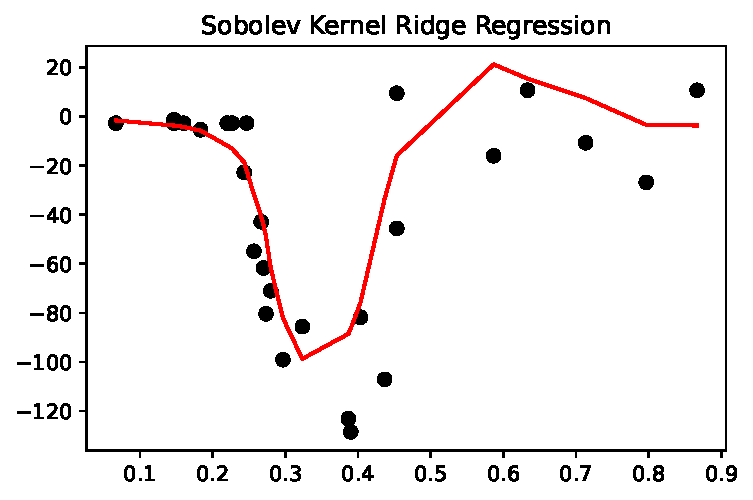
\includegraphics[keepaspectratio]{Tp2_files/figure-pdf/cell-14-output-3.pdf}}

\section{Activity 2 : Support Vector
Machine}\label{activity-2-support-vector-machine}

The support vector machines (SVM) is a supervised learning algorithm
that can be used for classification. The SVM is based on the concept of
finding the hyperplane that best separates the data into two classes. In
fact, if the problem is \textbf{linearly separable}, the SVM finds the
hyperplane that maximizes the margin between the two classes. The margin
is the distance between the hyperplane and the closest point of each
class (support vectors).

When the problem is non-linearly separable, the SVM uses the same
functionnement but allows some points to be misclassified. When the
problem is too complex, the SVM uses the kernel trick to transform the
data into a higher-dimensional space where the relationship is linear.

\subsection{I. Toy dataset}\label{i.-toy-dataset}

Here is the toy dataset that we are going to use to illustrate the SVM.
The dataset is composed of two features and the target variable is
binary. As we can see, the dataset is not linearly separable. We are
going to use the SVM with a gaussian kernel to classify the data, and
compare it to a classic classifier such as the k-nearest neighbors and
the logistic regression.

\begin{Shaded}
\begin{Highlighting}[]
\NormalTok{two\_moon\_data }\OperatorTok{=}\NormalTok{ pd.read\_csv(}\StringTok{"Data/DataTwoMoons.csv"}\NormalTok{,header}\OperatorTok{=}\VariableTok{None}\NormalTok{)}
\NormalTok{two\_moon\_data.columns }\OperatorTok{=}\NormalTok{ [}\StringTok{"X1"}\NormalTok{,}\StringTok{"X2"}\NormalTok{,}\StringTok{"y"}\NormalTok{]}

\NormalTok{plt.scatter(two\_moon\_data[}\StringTok{"X1"}\NormalTok{], two\_moon\_data[}\StringTok{"X2"}\NormalTok{], c}\OperatorTok{=}\NormalTok{two\_moon\_data[}\StringTok{"y"}\NormalTok{])}
\NormalTok{plt.title(}\StringTok{"Two moons dataset"}\NormalTok{)}
\end{Highlighting}
\end{Shaded}

\begin{verbatim}
Text(0.5, 1.0, 'Two moons dataset')
\end{verbatim}

\pandocbounded{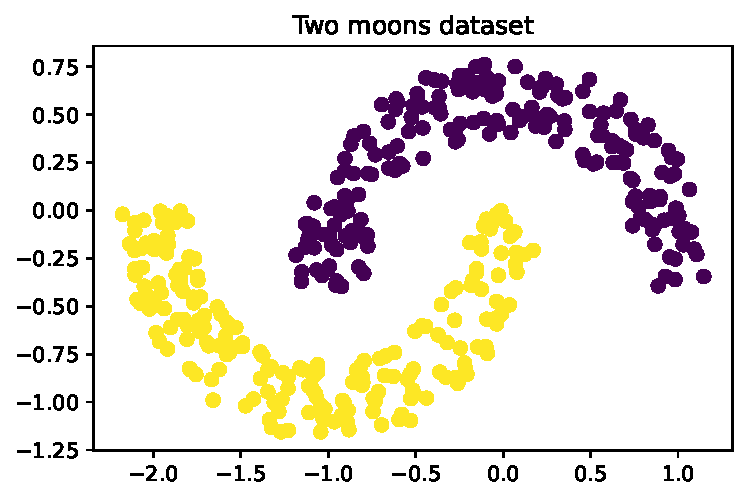
\includegraphics[keepaspectratio]{Tp2_files/figure-pdf/cell-15-output-2.pdf}}

\begin{Shaded}
\begin{Highlighting}[]
\CommentTok{\# Split the data into train and test sample}
\NormalTok{X\_train, X\_test, y\_train, y\_test }\OperatorTok{=}\NormalTok{ train\_test\_split(two\_moon\_data[[}\StringTok{"X1"}\NormalTok{,}\StringTok{"X2"}\NormalTok{]], two\_moon\_data[}\StringTok{"y"}\NormalTok{], test\_size}\OperatorTok{=}\FloatTok{0.2}\NormalTok{, random\_state}\OperatorTok{=}\DecValTok{42}\NormalTok{)}
\end{Highlighting}
\end{Shaded}

\subsubsection{1. K-nearest neighbors}\label{k-nearest-neighbors}

\begin{Shaded}
\begin{Highlighting}[]
\CommentTok{\# KNN with cross validation}

\NormalTok{knn }\OperatorTok{=}\NormalTok{ KNeighborsClassifier()}
\NormalTok{param\_grid }\OperatorTok{=}\NormalTok{ \{}\StringTok{"n\_neighbors"}\NormalTok{: np.arange(}\DecValTok{1}\NormalTok{, }\DecValTok{50}\NormalTok{)\}}
\NormalTok{knn\_cv }\OperatorTok{=}\NormalTok{ GridSearchCV(knn, param\_grid).fit(X\_train, y\_train)}
\BuiltInTok{print}\NormalTok{(}\SpecialStringTok{f"Best parameters by CV : }\SpecialCharTok{\{}\NormalTok{knn\_cv}\SpecialCharTok{.}\NormalTok{best\_params\_}\SpecialCharTok{\}}\SpecialStringTok{"}\NormalTok{)}

\CommentTok{\# Compute the accuracy}
\NormalTok{y\_pred }\OperatorTok{=}\NormalTok{ knn\_cv.predict(X\_test)}
\NormalTok{accuracy }\OperatorTok{=}\NormalTok{ accuracy\_score(y\_test, y\_pred)}
\BuiltInTok{print}\NormalTok{(}\SpecialStringTok{f"Accuracy: }\SpecialCharTok{\{}\NormalTok{accuracy}\SpecialCharTok{:.2f\}}\SpecialStringTok{"}\NormalTok{)}

\CommentTok{\# Confusion matrix to see detailed classification performance}
\NormalTok{conf\_matrix }\OperatorTok{=}\NormalTok{ confusion\_matrix(y\_test, y\_pred)}
\BuiltInTok{print}\NormalTok{(}\StringTok{"Confusion Matrix:"}\NormalTok{)}
\BuiltInTok{print}\NormalTok{(conf\_matrix)}

\CommentTok{\# Classification report for detailed metrics}
\BuiltInTok{print}\NormalTok{(}\StringTok{"Classification Report:"}\NormalTok{)}
\BuiltInTok{print}\NormalTok{(classification\_report(y\_test, y\_pred))}
\end{Highlighting}
\end{Shaded}

\begin{verbatim}
Best parameters by CV : {'n_neighbors': np.int64(1)}
Accuracy: 1.00
Confusion Matrix:
[[44  0]
 [ 0 36]]
Classification Report:
              precision    recall  f1-score   support

           0       1.00      1.00      1.00        44
           1       1.00      1.00      1.00        36

    accuracy                           1.00        80
   macro avg       1.00      1.00      1.00        80
weighted avg       1.00      1.00      1.00        80
\end{verbatim}

\begin{Shaded}
\begin{Highlighting}[]
\NormalTok{disp\_knn }\OperatorTok{=}\NormalTok{ DecisionBoundaryDisplay.from\_estimator(}
\NormalTok{    knn\_cv,}
\NormalTok{    X\_train,}
\NormalTok{    response\_method}\OperatorTok{=}\StringTok{"predict"}\NormalTok{,}
\NormalTok{    alpha }\OperatorTok{=} \FloatTok{0.3}
\NormalTok{)}
\NormalTok{disp\_knn.ax\_.scatter(two\_moon\_data[}\StringTok{"X1"}\NormalTok{],two\_moon\_data[}\StringTok{"X2"}\NormalTok{], c}\OperatorTok{=}\NormalTok{two\_moon\_data[}\StringTok{"y"}\NormalTok{])}
\NormalTok{plt.title(}\StringTok{"KNN Decision Boundary"}\NormalTok{)}
\NormalTok{plt.show()}
\end{Highlighting}
\end{Shaded}

\pandocbounded{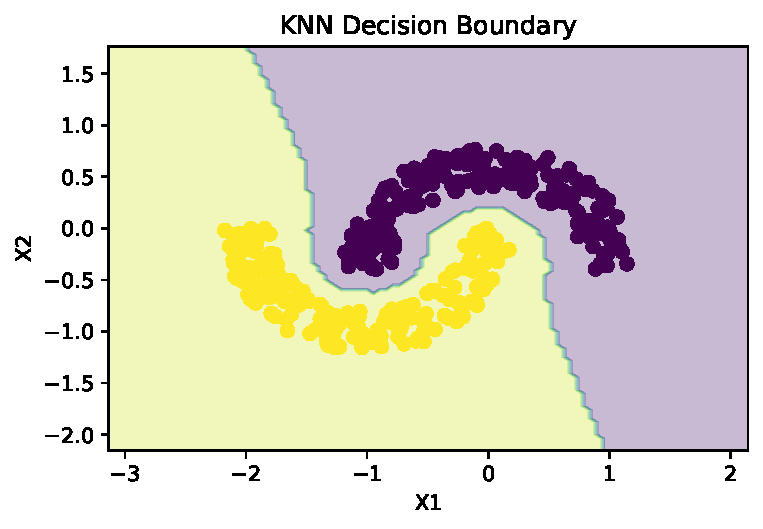
\includegraphics[keepaspectratio]{Tp2_files/figure-pdf/cell-18-output-1.pdf}}

\subsubsection{2. Logistic regression}\label{logistic-regression}

\begin{Shaded}
\begin{Highlighting}[]
\CommentTok{\# compute logistic regression}
\NormalTok{log\_reg }\OperatorTok{=}\NormalTok{ LogisticRegression(max\_iter}\OperatorTok{=}\DecValTok{1000}\NormalTok{)}
\NormalTok{log\_reg.fit(X\_train, y\_train)}
\NormalTok{y\_pred }\OperatorTok{=}\NormalTok{ log\_reg.predict(X\_test)}

\NormalTok{accuracy }\OperatorTok{=}\NormalTok{ accuracy\_score(y\_test, y\_pred)}
\BuiltInTok{print}\NormalTok{(}\SpecialStringTok{f"Accuracy: }\SpecialCharTok{\{}\NormalTok{accuracy}\SpecialCharTok{:.2f\}}\SpecialStringTok{"}\NormalTok{)}

\CommentTok{\# Confusion matrix to see detailed classification performance}
\NormalTok{conf\_matrix }\OperatorTok{=}\NormalTok{ confusion\_matrix(y\_test, y\_pred)}
\BuiltInTok{print}\NormalTok{(}\StringTok{"Confusion Matrix:"}\NormalTok{)}
\BuiltInTok{print}\NormalTok{(conf\_matrix)}

\CommentTok{\# Classification report for detailed metrics}
\BuiltInTok{print}\NormalTok{(}\StringTok{"Classification Report:"}\NormalTok{)}
\BuiltInTok{print}\NormalTok{(classification\_report(y\_test, y\_pred))}
\end{Highlighting}
\end{Shaded}

\begin{verbatim}
Accuracy: 0.91
Confusion Matrix:
[[39  5]
 [ 2 34]]
Classification Report:
              precision    recall  f1-score   support

           0       0.95      0.89      0.92        44
           1       0.87      0.94      0.91        36

    accuracy                           0.91        80
   macro avg       0.91      0.92      0.91        80
weighted avg       0.92      0.91      0.91        80
\end{verbatim}

\begin{Shaded}
\begin{Highlighting}[]
\NormalTok{disp\_log\_reg }\OperatorTok{=}\NormalTok{ DecisionBoundaryDisplay.from\_estimator(}
\NormalTok{    log\_reg,}
\NormalTok{    X\_train,}
\NormalTok{    response\_method}\OperatorTok{=}\StringTok{"predict"}\NormalTok{,}
\NormalTok{    alpha }\OperatorTok{=} \FloatTok{0.3}
\NormalTok{)}
\NormalTok{disp\_log\_reg.ax\_.scatter(two\_moon\_data[}\StringTok{"X1"}\NormalTok{],two\_moon\_data[}\StringTok{"X2"}\NormalTok{], c}\OperatorTok{=}\NormalTok{two\_moon\_data[}\StringTok{"y"}\NormalTok{], edgecolor}\OperatorTok{=}\StringTok{"k"}\NormalTok{)}
\NormalTok{plt.title(}\StringTok{"Logistic Regression Decision Boundary"}\NormalTok{)}
\NormalTok{plt.show()}
\end{Highlighting}
\end{Shaded}

\pandocbounded{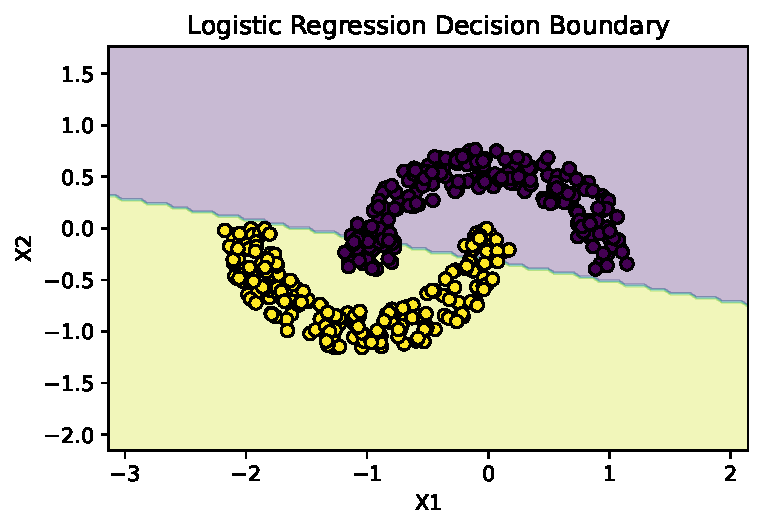
\includegraphics[keepaspectratio]{Tp2_files/figure-pdf/cell-20-output-1.pdf}}

\subsubsection{3. SVM}\label{svm}

\begin{Shaded}
\begin{Highlighting}[]
\NormalTok{grid\_eval }\OperatorTok{=}\NormalTok{ np.logspace(}\OperatorTok{{-}}\DecValTok{2}\NormalTok{, }\DecValTok{4}\NormalTok{, }\DecValTok{50}\NormalTok{)}
\NormalTok{param\_grid }\OperatorTok{=}\NormalTok{ \{}\StringTok{"C"}\NormalTok{: grid\_eval, }\StringTok{"gamma"}\NormalTok{: grid\_eval\}}
\NormalTok{svm\_model }\OperatorTok{=}\NormalTok{ SVC(kernel}\OperatorTok{=}\StringTok{"rbf"}\NormalTok{)}
\NormalTok{svm\_model\_cv }\OperatorTok{=}\NormalTok{ GridSearchCV(svm\_model, param\_grid).fit(X\_train,y\_train)}
\BuiltInTok{print}\NormalTok{(}\SpecialStringTok{f"Best parameters by CV : }\SpecialCharTok{\{}\NormalTok{svm\_model\_cv}\SpecialCharTok{.}\NormalTok{best\_params\_}\SpecialCharTok{\}}\SpecialStringTok{"}\NormalTok{)}
\end{Highlighting}
\end{Shaded}

\begin{verbatim}
Best parameters by CV : {'C': np.float64(0.030888435964774818), 'gamma': np.float64(3.727593720314938)}
\end{verbatim}

\begin{Shaded}
\begin{Highlighting}[]
\CommentTok{\# Compute the accuracy}
\NormalTok{y\_pred }\OperatorTok{=}\NormalTok{ svm\_model\_cv.predict(X\_test)}
\NormalTok{accuracy }\OperatorTok{=}\NormalTok{ accuracy\_score(y\_test, y\_pred)}
\BuiltInTok{print}\NormalTok{(}\SpecialStringTok{f"Accuracy: }\SpecialCharTok{\{}\NormalTok{accuracy}\SpecialCharTok{:.2f\}}\SpecialStringTok{"}\NormalTok{)}

\CommentTok{\# Confusion matrix to see detailed classification performance}
\NormalTok{conf\_matrix }\OperatorTok{=}\NormalTok{ confusion\_matrix(y\_test, y\_pred)}
\BuiltInTok{print}\NormalTok{(}\StringTok{"Confusion Matrix:"}\NormalTok{)}
\BuiltInTok{print}\NormalTok{(conf\_matrix)}

\CommentTok{\# Classification report for detailed metrics}
\BuiltInTok{print}\NormalTok{(}\StringTok{"Classification Report:"}\NormalTok{)}
\BuiltInTok{print}\NormalTok{(classification\_report(y\_test, y\_pred))}
\end{Highlighting}
\end{Shaded}

\begin{verbatim}
Accuracy: 1.00
Confusion Matrix:
[[44  0]
 [ 0 36]]
Classification Report:
              precision    recall  f1-score   support

           0       1.00      1.00      1.00        44
           1       1.00      1.00      1.00        36

    accuracy                           1.00        80
   macro avg       1.00      1.00      1.00        80
weighted avg       1.00      1.00      1.00        80
\end{verbatim}

\begin{Shaded}
\begin{Highlighting}[]
\NormalTok{disp\_svm }\OperatorTok{=}\NormalTok{ DecisionBoundaryDisplay.from\_estimator(}
\NormalTok{    svm\_model\_cv,}
\NormalTok{    X\_train,}
\NormalTok{    response\_method}\OperatorTok{=}\StringTok{"predict"}\NormalTok{,}
\NormalTok{    alpha }\OperatorTok{=} \FloatTok{0.3}
\NormalTok{)}
\NormalTok{disp\_svm.ax\_.scatter(two\_moon\_data[}\StringTok{"X1"}\NormalTok{],two\_moon\_data[}\StringTok{"X2"}\NormalTok{], c}\OperatorTok{=}\NormalTok{two\_moon\_data[}\StringTok{"y"}\NormalTok{], edgecolor}\OperatorTok{=}\StringTok{"k"}\NormalTok{)}
\NormalTok{plt.title(}\StringTok{"SVM Decision Boundary"}\NormalTok{)}
\NormalTok{plt.show()}
\end{Highlighting}
\end{Shaded}

\pandocbounded{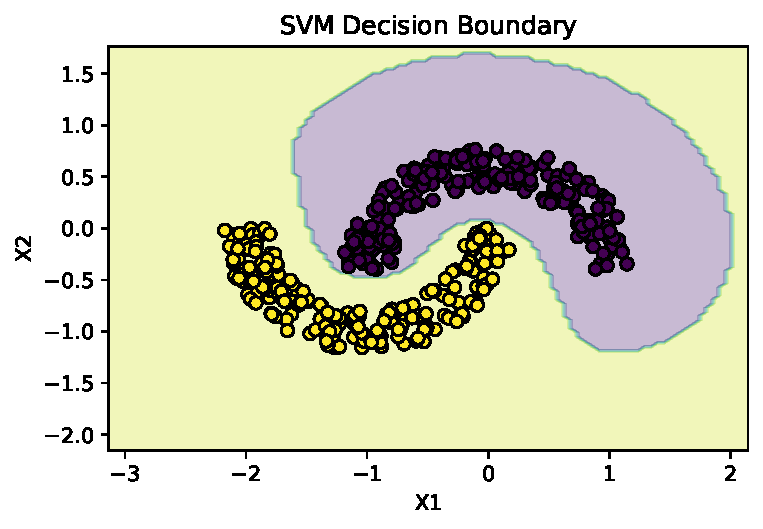
\includegraphics[keepaspectratio]{Tp2_files/figure-pdf/cell-23-output-1.pdf}}

\subsubsection{4. Conclusion}\label{conclusion}

As we can see, the SVM with the gaussian kernel is able to classify the
data with a good accuracy. The SVM is able to capture the non-linear
relationship between the target variable and the features.

The logistic regression, in this case, is not able to classify the data
because the relationship between the target variable and the features is
non-linear.

The k-nearest neighbors is able to classify the data with a performance
similar to the SVM. The SVM and the KNN are a good choice when we have a
non-linear relationship between the target variable and the features.

\textbf{Whenever we have a classification problem, it is hence always
useful to try the SVM and the KNN.}

\subsection{II. Image dataset}\label{ii.-image-dataset}

The SVM is also useful for image classification. In this part, we are
going to use the famous MNIST dataset to classify the images. The MNIST
dataset is composed of 20 000 images (10 000 in the training dataset,
and 10 000 also in the test dataset) of handwritten digits from 0 to 9.
Each image is a resolution 28x28 pixels that is represented by a matrix
of shape (28, 28), with each element being the pixel intensity (values
from 0 to 255). We are going to use the SVM with the gaussian kernel to
classify the images.

We will start by normalizing the data to ensure that all the features
contribute equally, and then use the GridSearchCV function from
scikit-learn to find the best hyperparameter.

\begin{Shaded}
\begin{Highlighting}[]
\NormalTok{data\_train }\OperatorTok{=}\NormalTok{ pd.read\_csv(}\StringTok{"Data/mnist\_train\_small.csv"}\NormalTok{)}
\NormalTok{data\_test }\OperatorTok{=}\NormalTok{ pd.read\_csv(}\StringTok{"Data/mnist\_test.csv"}\NormalTok{)}

\BuiltInTok{print}\NormalTok{(}\StringTok{"Description of train dataset : }\CharTok{\textbackslash{}n}\StringTok{"}\NormalTok{)}
\NormalTok{data\_train.iloc[:,}\DecValTok{1}\NormalTok{:].describe()}
\NormalTok{data\_train[}\StringTok{"label"}\NormalTok{].value\_counts()}
\end{Highlighting}
\end{Shaded}

\begin{verbatim}
Description of train dataset : 
\end{verbatim}

\begin{verbatim}
label
8    113
0    111
1    110
7    106
9    100
2     99
4     95
5     93
6     90
3     83
Name: count, dtype: int64
\end{verbatim}

\begin{Shaded}
\begin{Highlighting}[]
\CommentTok{\# normalize the data}
\ImportTok{from}\NormalTok{ sklearn.preprocessing }\ImportTok{import}\NormalTok{ StandardScaler}
\NormalTok{scaler }\OperatorTok{=}\NormalTok{ StandardScaler()}

\NormalTok{X\_train  }\OperatorTok{=}\NormalTok{ scaler.fit\_transform(data\_train.iloc[:, }\DecValTok{1}\NormalTok{:])}
\NormalTok{y\_train }\OperatorTok{=}\NormalTok{ data\_train[}\StringTok{"label"}\NormalTok{]}
\NormalTok{X\_test  }\OperatorTok{=}\NormalTok{ scaler.transform(data\_test.iloc[:, }\DecValTok{1}\NormalTok{:])}
\NormalTok{y\_test }\OperatorTok{=}\NormalTok{ data\_test[}\StringTok{"label"}\NormalTok{]}
\end{Highlighting}
\end{Shaded}

As we can see from the umap plot, which is a dimensionality reduction
technique, the data is not always linearly separable. We are going to
use the SVM with the gaussian kernel to classify the images.

\begin{Shaded}
\begin{Highlighting}[]
\CommentTok{\# visualize the data with UMAP}
\NormalTok{reducer }\OperatorTok{=}\NormalTok{ umap.UMAP(random\_state}\OperatorTok{=}\DecValTok{42}\NormalTok{)}
\NormalTok{embedding }\OperatorTok{=}\NormalTok{ reducer.fit\_transform(X\_train)}
\end{Highlighting}
\end{Shaded}

\begin{Shaded}
\begin{Highlighting}[]
\NormalTok{plt.scatter(embedding[:, }\DecValTok{0}\NormalTok{], embedding[:, }\DecValTok{1}\NormalTok{], c}\OperatorTok{=}\NormalTok{data\_train[}\StringTok{"label"}\NormalTok{], cmap}\OperatorTok{=}\StringTok{\textquotesingle{}Spectral\textquotesingle{}}\NormalTok{, s}\OperatorTok{=}\DecValTok{1}\NormalTok{)}
\NormalTok{plt.gca().set\_aspect(}\StringTok{\textquotesingle{}equal\textquotesingle{}}\NormalTok{, }\StringTok{\textquotesingle{}datalim\textquotesingle{}}\NormalTok{)}
\NormalTok{plt.colorbar()}
\NormalTok{plt.title(}\StringTok{\textquotesingle{}UMAP projection of the MNIST dataset\textquotesingle{}}\NormalTok{)}
\end{Highlighting}
\end{Shaded}

\begin{verbatim}
Text(0.5, 1.0, 'UMAP projection of the MNIST dataset')
\end{verbatim}

\pandocbounded{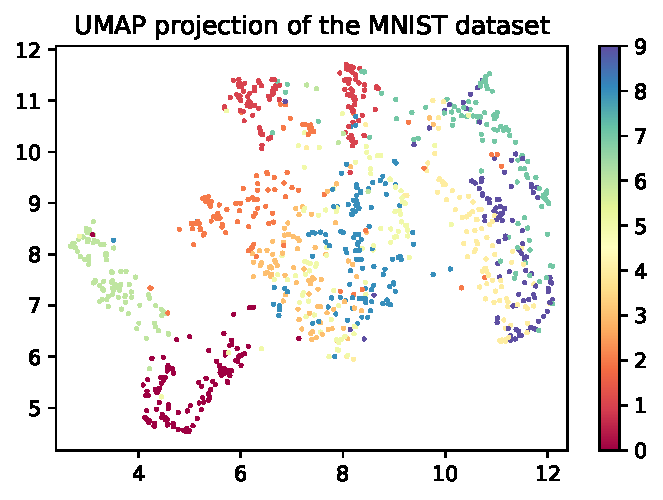
\includegraphics[keepaspectratio]{Tp2_files/figure-pdf/cell-27-output-2.pdf}}

\begin{Shaded}
\begin{Highlighting}[]
\NormalTok{svm\_model }\OperatorTok{=}\NormalTok{ SVC(kernel}\OperatorTok{=}\StringTok{"rbf"}\NormalTok{)}
\ImportTok{from}\NormalTok{ itertools }\ImportTok{import}\NormalTok{ product}

\NormalTok{grid\_eval\_C }\OperatorTok{=}\NormalTok{ [c }\OperatorTok{*}\NormalTok{ factor }\ControlFlowTok{for}\NormalTok{ c, factor }\KeywordTok{in}\NormalTok{ product([}\FloatTok{0.1}\NormalTok{, }\DecValTok{1}\NormalTok{, }\DecValTok{10}\NormalTok{], [}\DecValTok{1}\NormalTok{, }\DecValTok{5}\NormalTok{])]}
\NormalTok{grid\_eval\_gamma }\OperatorTok{=}\NormalTok{ [gamma }\OperatorTok{*}\NormalTok{ factor }\ControlFlowTok{for}\NormalTok{ gamma, factor }\KeywordTok{in}\NormalTok{ product([}\DecValTok{10}\OperatorTok{**{-}}\DecValTok{3}\NormalTok{, }\DecValTok{10}\OperatorTok{**{-}}\DecValTok{2}\NormalTok{, }\DecValTok{10}\OperatorTok{**{-}}\DecValTok{1}\NormalTok{], [}\DecValTok{1}\NormalTok{, }\DecValTok{5}\NormalTok{])]}


\NormalTok{param\_grid }\OperatorTok{=}\NormalTok{ \{}\StringTok{"C"}\NormalTok{: grid\_eval\_C, }\StringTok{"gamma"}\NormalTok{: grid\_eval\_gamma\}}
\NormalTok{svm\_model\_cv }\OperatorTok{=}\NormalTok{ GridSearchCV(svm\_model, param\_grid).fit(X\_train, y\_train)}
\BuiltInTok{print}\NormalTok{(}\SpecialStringTok{f"Best parameters by CV : }\SpecialCharTok{\{}\NormalTok{svm\_model\_cv}\SpecialCharTok{.}\NormalTok{best\_params\_}\SpecialCharTok{\}}\SpecialStringTok{"}\NormalTok{)}
\end{Highlighting}
\end{Shaded}

\begin{verbatim}
Best parameters by CV : {'C': 5, 'gamma': 0.001}
\end{verbatim}

As we can see, the model performs well with an accuracy of 0.88 . As
expected from the umap visualization, the model is able to separate the
classes well, however there are some errors in the classification. The
confusion matrix shows that the model has some difficulty to distinguish
between some digits such as 4 and 9, 3.

The SVM is a good choice for image classification, however, the model is
not able to capture the complexity of the data. In this case, we can use
a deep learning model such as the convolutional neural network (CNN)
which is able to capture the complexity of the data.

\begin{Shaded}
\begin{Highlighting}[]
\CommentTok{\# compute the accuracy}
\NormalTok{y\_pred }\OperatorTok{=}\NormalTok{ svm\_model\_cv.predict(X\_test)}
\NormalTok{accuracy }\OperatorTok{=}\NormalTok{ accuracy\_score(y\_test, y\_pred)}
\BuiltInTok{print}\NormalTok{(}\SpecialStringTok{f"Accuracy: }\SpecialCharTok{\{}\NormalTok{accuracy}\SpecialCharTok{:.2f\}}\SpecialStringTok{"}\NormalTok{)}

\CommentTok{\# Confusion matrix to see detailed classification performance}
\NormalTok{conf\_matrix }\OperatorTok{=}\NormalTok{ confusion\_matrix(y\_test, y\_pred)}
\BuiltInTok{print}\NormalTok{(}\StringTok{"Confusion Matrix:"}\NormalTok{)}
\BuiltInTok{print}\NormalTok{(conf\_matrix)}

\CommentTok{\# Classification report for detailed metrics}
\BuiltInTok{print}\NormalTok{(}\StringTok{"Classification Report:"}\NormalTok{)}
\BuiltInTok{print}\NormalTok{(classification\_report(y\_test, y\_pred))}
\end{Highlighting}
\end{Shaded}

\begin{verbatim}
Accuracy: 0.88
Confusion Matrix:
[[ 931    0   20    1    1   12    9    2    4    0]
 [   0 1121    4    2    0    1    6    0    1    0]
 [  14    6  949   20    7    2    6   10   17    1]
 [   6    2   75  829    2   29    3   30   25    9]
 [   3    5   32    0  881    3    9    4    5   40]
 [   4    3   75   31    5  718   20    9   16   11]
 [  20    5  101    0    8   11  808    0    5    0]
 [   1   12   61    1   10    2    0  913    0   28]
 [   8   14   37   13   11   23    5   18  829   16]
 [   9    6   30   12   37    4    0   57    1  853]]
Classification Report:
              precision    recall  f1-score   support

           0       0.93      0.95      0.94       980
           1       0.95      0.99      0.97      1135
           2       0.69      0.92      0.79      1032
           3       0.91      0.82      0.86      1010
           4       0.92      0.90      0.91       982
           5       0.89      0.80      0.85       892
           6       0.93      0.84      0.89       958
           7       0.88      0.89      0.88      1028
           8       0.92      0.85      0.88       974
           9       0.89      0.85      0.87      1009

    accuracy                           0.88     10000
   macro avg       0.89      0.88      0.88     10000
weighted avg       0.89      0.88      0.88     10000
\end{verbatim}

\begin{Shaded}
\begin{Highlighting}[]
\CommentTok{\# plot ROC CURVE}
\ImportTok{from}\NormalTok{ sklearn.metrics }\ImportTok{import}\NormalTok{ roc\_curve, auc}
\ImportTok{from}\NormalTok{ sklearn.preprocessing }\ImportTok{import}\NormalTok{ label\_binarize}

\NormalTok{y\_test\_bin }\OperatorTok{=}\NormalTok{ label\_binarize(y\_test, classes}\OperatorTok{=}\NormalTok{[}\DecValTok{0}\NormalTok{, }\DecValTok{1}\NormalTok{, }\DecValTok{2}\NormalTok{, }\DecValTok{3}\NormalTok{, }\DecValTok{4}\NormalTok{, }\DecValTok{5}\NormalTok{, }\DecValTok{6}\NormalTok{, }\DecValTok{7}\NormalTok{, }\DecValTok{8}\NormalTok{, }\DecValTok{9}\NormalTok{])}
\NormalTok{y\_score }\OperatorTok{=}\NormalTok{ svm\_model\_cv.decision\_function(X\_test)}
\NormalTok{fpr }\OperatorTok{=} \BuiltInTok{dict}\NormalTok{()}
\NormalTok{tpr }\OperatorTok{=} \BuiltInTok{dict}\NormalTok{()}
\NormalTok{roc\_auc }\OperatorTok{=} \BuiltInTok{dict}\NormalTok{()}
\ControlFlowTok{for}\NormalTok{ i }\KeywordTok{in} \BuiltInTok{range}\NormalTok{(}\DecValTok{10}\NormalTok{):}
\NormalTok{    fpr[i], tpr[i], \_ }\OperatorTok{=}\NormalTok{ roc\_curve(y\_test\_bin[:, i], y\_score[:, i])}
\NormalTok{    roc\_auc[i] }\OperatorTok{=}\NormalTok{ auc(fpr[i], tpr[i])}

\NormalTok{plt.figure()}
\NormalTok{colors }\OperatorTok{=}\NormalTok{ [}\StringTok{\textquotesingle{}blue\textquotesingle{}}\NormalTok{, }\StringTok{\textquotesingle{}red\textquotesingle{}}\NormalTok{, }\StringTok{\textquotesingle{}green\textquotesingle{}}\NormalTok{, }\StringTok{\textquotesingle{}orange\textquotesingle{}}\NormalTok{, }\StringTok{\textquotesingle{}purple\textquotesingle{}}\NormalTok{, }\StringTok{\textquotesingle{}brown\textquotesingle{}}\NormalTok{, }\StringTok{\textquotesingle{}pink\textquotesingle{}}\NormalTok{, }\StringTok{\textquotesingle{}gray\textquotesingle{}}\NormalTok{, }\StringTok{\textquotesingle{}olive\textquotesingle{}}\NormalTok{, }\StringTok{\textquotesingle{}cyan\textquotesingle{}}\NormalTok{]}
\ControlFlowTok{for}\NormalTok{ i, color }\KeywordTok{in} \BuiltInTok{zip}\NormalTok{(}\BuiltInTok{range}\NormalTok{(}\DecValTok{10}\NormalTok{), colors):}
\NormalTok{    plt.plot(fpr[i], tpr[i], color}\OperatorTok{=}\NormalTok{color, lw}\OperatorTok{=}\DecValTok{2}\NormalTok{, label}\OperatorTok{=}\SpecialStringTok{f\textquotesingle{}Class }\SpecialCharTok{\{}\NormalTok{i}\SpecialCharTok{\}}\SpecialStringTok{ (AUC =}\SpecialCharTok{\{}\NormalTok{roc\_auc[i]}\SpecialCharTok{:.2f\}}\SpecialStringTok{)\textquotesingle{}}\NormalTok{)}
\NormalTok{plt.plot([}\DecValTok{0}\NormalTok{, }\DecValTok{1}\NormalTok{], [}\DecValTok{0}\NormalTok{, }\DecValTok{1}\NormalTok{], }\StringTok{\textquotesingle{}k{-}{-}\textquotesingle{}}\NormalTok{, lw}\OperatorTok{=}\DecValTok{2}\NormalTok{)}
\NormalTok{plt.xlim([}\FloatTok{0.0}\NormalTok{, }\FloatTok{1.0}\NormalTok{])}
\NormalTok{plt.ylim([}\FloatTok{0.0}\NormalTok{, }\FloatTok{1.05}\NormalTok{])}
\NormalTok{plt.xlabel(}\StringTok{\textquotesingle{}False Positive Rate\textquotesingle{}}\NormalTok{)}
\NormalTok{plt.ylabel(}\StringTok{\textquotesingle{}True Positive Rate\textquotesingle{}}\NormalTok{)}
\NormalTok{plt.title(}\StringTok{\textquotesingle{}ROC Curve\textquotesingle{}}\NormalTok{)}
\NormalTok{plt.legend(loc}\OperatorTok{=}\StringTok{"lower right"}\NormalTok{)}
\NormalTok{plt.show()}
\end{Highlighting}
\end{Shaded}

\pandocbounded{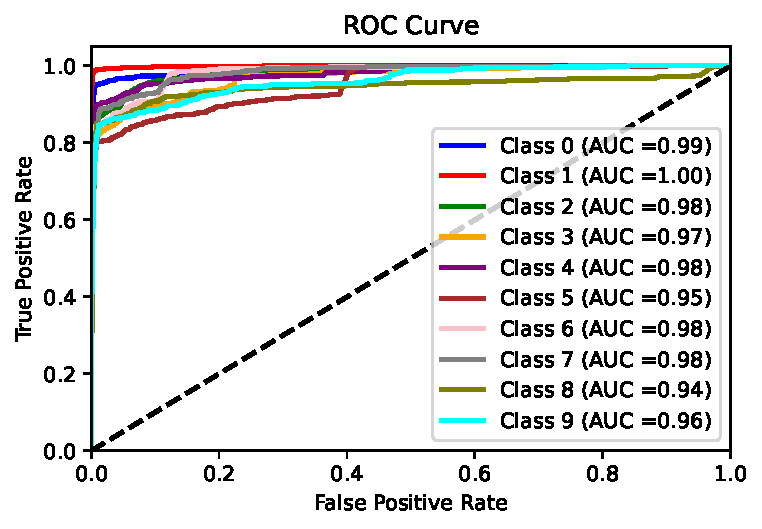
\includegraphics[keepaspectratio]{Tp2_files/figure-pdf/cell-30-output-1.pdf}}




\end{document}
